\chapter{The Nature of LAPD Turbulence}
\label{c_lapd_turb}

\section{LAPD Linear Instabilities}
\label{s_lin_inst}

Linear instabilities are prevalent in plasma physics. They come from the linearization around an equilibrium of the plasma equations. Physically, if a plasma is in a time-independent
steady state that is linearly unstable and a finite fluctuation of any size occurs, the fluctuation will grow exponentially.
The LAPD equations, parameters, and profiles described in Chapter~\ref{c_lapd_sim} give rise to a couple of linear instabilities. They are both drift wave type instabilities, but they 
have different pressure/potential coupling mechanisms. One type couples through the adiabatic response, while the other couples through the sheath boundary response.

\subsection{Drift Waves}
\label{ss_drift_waves}

Electron drift waves driven by an equilibrium density or pressure gradient that use the adiabatic response are generally referred to as just drift waves or the universal instability.
The electron drift wave mechanism is the following: An electron pressure fluctuation in the plasma is linked with a potential fluctuation through the adiabatic response. The adiabatic
response is simply a parallel force balance between the pressure force and the electrostatic force. A simplified version of Eq.~\ref{brag_mom} can be written:

\beq
\label{adiabatic_response}
\gradpar p_e = e n \gradpar \phi + R \vpe,
\eeq

where the term $R \vpe$ represents effects such as electron inertia, resistivity, and electromagnetic induction. If $R=0$, the electrons are said to be adiabatic, meaning 
$\gradpar p_e = e n \gradpar \phi$. When $T_e$ fluctuations are neglected and $\gradpar \ne 0$, this integrates to the Boltzmann expression:

\beq
\label{boltzmann_exp}
n = n_0 e^{e \phi/T_e}.
\eeq

For any $R$ and $T_e$ fluctuations, the parallel electron dynamics couple the pressure to the potential as long as the parallel wavelength $k_\para$ is finite. 
The perpendicular electric field associated with the potential fluctuation has a component in the azimuthal direction with $k_\perp \gg k_\para$. 
This creates a radial ${\bf E \times B}$ drift that advects the pressure in the radial direction. Because of the radial pressure gradient,
the fluctuation to propagates azimuthally as a wave at the drift speed $v_{De} = \frac{T_e}{e B} \pdiff{{\rm ln} N_0}{r}$~\cite{chen2006} in the electron diamagnetic drift direction. 
If there is a small phase difference between the pressure and the potential of the wave (the result of $R \ne 0$), the equilibrium pressure gradient will enhance the fluctuation, causing
instability. Since $p_e = n_e T_e$, the pressure fluctuation may be due to either a density fluctuation, an electron temperature fluctuation, or both. The universal instability generally
refers to the situation where an equilibrium density gradient drives a density fluctuating wave. But a temperature gradient driving a temperature fluctuation wave is also possible, and
may be called a thermal drift wave~\cite{makwana2011}. It's not necessary, however, to separate them, and we will just refer to both of these as drift waves.

\begin{figure}[!htbp]
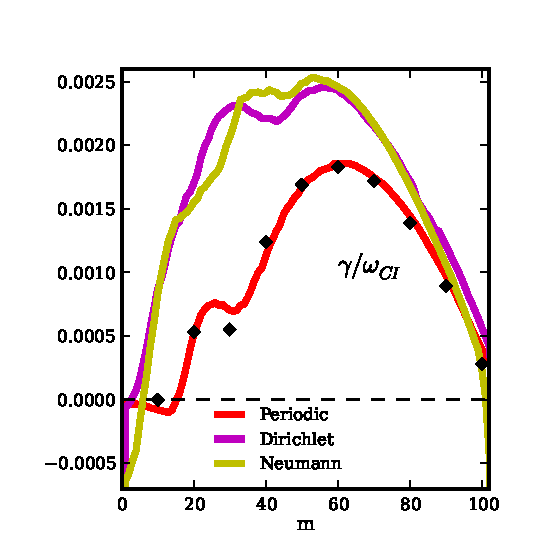
\includegraphics[]{lin_dw_gamma}
\hfil
\caption{Linear drift wave a) growth rates and b) axial structures}
\label{lin_dw_gamma}
\end{figure}

The LAPD equation set (Eqs.~\ref{ni_eq}-\ref{te_eq}) supports such drift waves, which are unstable with the parameters and profiles used in the simulations. 
The growth rate as a function of the azimuthal
wavenumber $m$ is shown in Fig.~\ref{lin_dw_gamma} a) for the LAPD parameters in Table~\ref{parameter_table} and profiles in Fig.~\ref{equilibrium_profiles}. The growth rates are found by simulating
the linearized version of Eqs.~\ref{ni_eq}-\ref{te_eq} in BOUT++ with the three different simple axial boundary conditions: periodic, zero-value (Dirichlet), and zero-derivative (Neumann). 
The linear equations simply omit the advective nonlinearities and the source terms, though the source terms have no affect on any of the linear modes besides $m=0$ modes. The simulations are run
for long enough so that the fastest growing modes can dominate the dynamics.

The solid curves in Fig.~\ref{lin_dw_gamma} are calculated from the simulation results using the formula, $\gamma_m = \pdiff{E_m}{t}/(2 E_m)$ where $E_m$ is the energy of the fastest
growing linear eigenmode with azimuthal mode number $m$.
The energy is defined in Chapter~\ref{c_en_formalism}. The details of obtaining $\gamma_m$ are explained in that chapter, but for now, it is sufficient to state that this procedure calculates
$\gamma_m$ at a particular time using only the structures of the fluctuating quantities: $N, \phi, \vpe, {\rm and } T_e$. An alternative way to calculate $\gamma_m$ is to use BOUT++'s Fourier
filtering capabilities and run many simulations where each one filters out a different azimuthal mode. Then, we take the log of the envelope of one or several of the fluctuating quantities
and calculate the slope of the line, which gives the growth rate for each particular simulation. This procedure uses the time signal of the fluctuations rather than their spatial structure to
calculate the growth rate, thus providing a check on the first method. 
The results using this alternative method for the periodic case are shown with the black diamonds in Fig.~\ref{lin_dw_gamma} a), which agree well with the curve calculated using the 
alternative energetic structure-based calculation. We do this check with all of the simulations to ensure consistency. This second method is more time consuming, so we only sample a few values of $m$.
Furthermore, it's difficult to get growth rates when $\gamma_m < 0$ using this second method.

The difference in the growth rate curves with the different boundary conditions is due to the different $k_\para = \frac{2 \pi n}{L_\para}$ where $n$ is the axial mode number. The periodic simulation
restricts $n$ to integer values, while the Dirichlet and Neumann simulations allow for any fractional $n$. The largest growth rate occurs for $n \sim 1/2$. The Dirichlet and Neumann axial structures
for the most unstable $m$ mode, shown in Fig.~\ref{lin_dw_gamma} b), reflect this. The periodic simulation, which has $n=1$ structure, has a smaller growth rate, especially at low $m$. Note that in
Fig.~\ref{lin_dw_gamma} b), the axial boundaries are not plotted. For instance, the zero-valued boundaries for the Dirichlet simulation are not shown. Also, the axial structures are taken at one
random point in the $r-\theta$ plane and at one time point, and are normalized to their maximum value.

\subsection{Conducting Wall Mode}
\label{ss_cwm}

\begin{figure}[!htbp]
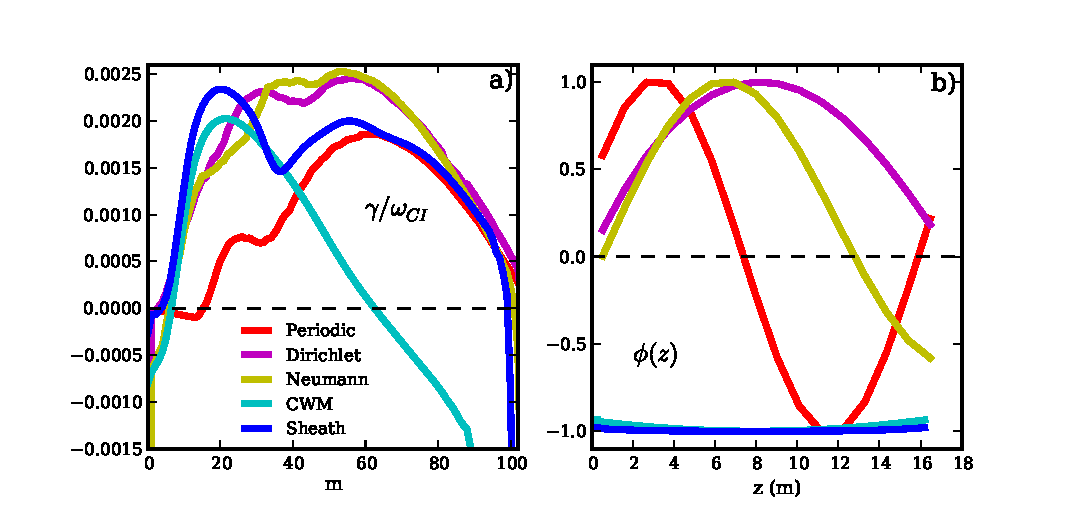
\includegraphics[]{lin_all_gamma}
\hfil
\caption{Linear conducting wall mode a) growth rates and b) axial structures}
\label{lin_all_gamma}
\end{figure}


We now consider the linear instability that can exist in a plasma bounded by two conducting walls on the boundaries where the magnetic field lines terminate
(the axial boundaries)~\cite{berk1991,berk1993,xu1993}.
The instability is actually of the drift wave variety, but unlike the drift waves discussed above, the pressure-potential coupling mechanism is through the sheath boundary response
rather than through the adiabatic response. The Bohm sheath boundary conditions that were derived in Sec.~\ref{ss_bs_bc} can provide this coupling. 
As already noted, these boundary conditions are not necessarily the correct ones
for LAPD, but are somewhat idealized. Yet, it is still academically instructive to apply such an idealized boundary condition to LAPD because it creates this new linear instability, which
can be used to test the robustness of LAPD's nonlinear instability.

The conducting wall mode (CWM) instability in the case considered here is purely an electron temperature gradient instability, although other types of gradients can cause it~\cite{berk1993}.
Electron temperature fluctuations are advected by electrostatic potential fluctuations and feed off the equilibrium electron temperature gradient as in the case of the thermal drift waves.
However, in contrast to the thermal drift waves, the coupling between the temperature and potential fluctuations comes through the sheath boundary condition rather than through the adiabatic
response. Furthermore, the CWM can have (nearly) $k_\para = 0$ flute-like behavior. The coupling mechanism is as follows: an electron temperature perturbation -- say a
positive constant fluctuation along a small flux tube -- increases the sound speed and the electron thermal speed on the flux tube. 
Since the ions must enter the Bohm sheath at the sound speed by being accelerated
by a parallel electric field, the temperature increase must coincide with an increase in the parallel potential gradient as derived in Eq.~\ref{sheath_bc}. Additionally, the increased
electron thermal speed causes an increase in the floating potential along the flux tube. These serve to couple the electron temperature to the potential.

The CWM can be isolated from the normal drift waves by removing the adiabatic response from the full LAPD equation set, and of course using the Bohm sheath boundary condition of Eq.~\ref{sheath_bc}.
Removal of the adiabatic response in this case means removal of the $\gradpar p_e$ and the $0.71 \gradpar T_e$ terms in the parallel momentum equation (Eq.~\ref{ve_eq}). This causes the 
density fluctuation $N$ to become a passive scalar, so Eq.~\ref{ni_eq} can be removed as well with no consequence. So the isolated linear CWM equations are:

\beqar
\label{ve_eq_cwm}
\pdt \vpe = \fmie \gradpar \phi - \nue \vpe, \\
\label{rho_eq_cwm}
\pdt \varpi = - N_0 \gradpar \vpe - \nuin \varpi + \mu_\phi \gradperp^2 \varpi, \\
\label{te_eq_cwm}
\pdt T_e = - {\mathbf v_E} \cdot \grad T_{e0} + \frac{2}{3 N_0} \kpe \gradpar^2 T_e  - \frac{2 m_e}{m_i} \nue T_e  + \mu_T \gradperp^2 T_e,
\eeqar

The CWM growth rate curve is shown in Fig.~\ref{lin_all_gamma} a). The CWM is most unstable at values of $m \sim 20$, which is much lower than the $m \sim 60$ values of the drift waves.
Furthermore, the CWM maximum growth rate is about equal to the drift wave growth rates. And from Fig.~\ref{lin_all_gamma} b), the CWM axial structure is flute-like ($k_\para \simeq 0$). 
Finally, the growth rate curve of the full set of equations along with the sheath boundary condition is shown in this figure as the curve labeled ``sheath.'' This set of equations contains
the drift wave and CWM instabilities. From both Figs.~\ref{lin_all_gamma} a) and b), it is clear that the sheath simulation is dominated by the CWM at $m \leq 20$, which in fact is where
the growth rate is maximum. At $m \geq 40$, the drift waves dominate.


\section{LAPD Turbulence: A Visual Examination}
\label{s_vis_exam}

\section{LAPD Turbulence: A Statistical Examination}
\label{s_stat_exam}

% Look at the spectra at different radial locations to determine if they're exponential

% Look at k-spectra
